\documentclass[a4paper]{article}

\usepackage[english]{babel}
\usepackage{amsfonts, amssymb, mathtools, amsthm, amsmath}
\usepackage{graphicx, pgfplots}
\usepackage{bm} 
\usepackage{url}
\usepackage[dvipsnames]{xcolor}
\usepackage{lastpage}
\usepackage{chngcntr}
  \counterwithin{figure}{section}
  \renewcommand{\thefigure}{\thesection.\arabic{figure}}

%loaded last
\usepackage[hidelinks]{hyperref}
\usepackage[nameinlink]{cleveref} 

\usepackage{siunitx}
  \sisetup{exponent-product = \cdot,
    output-decimal-marker = {,}}

%Giles Castelles incfig
\usepackage{import}
\usepackage{xifthen}
\usepackage{pdfpages}
\usepackage{transparent}

\newcommand{\incfig}[2][1]{%
  \def\svgwidth{#1\columnwidth}
  \import{./figures/}{#2.pdf_tex}
}

\setlength{\parindent}{0in}
\setlength{\parskip}{12pt}
\setlength{\oddsidemargin}{0in}
\setlength{\textwidth}{6.5in}
\setlength{\textheight}{8.8in}
\setlength{\topmargin}{0in}
\setlength{\headheight}{18pt}

\usepackage{fancyhdr}
\pagestyle{fancy}

\fancyhead{}
\fancyfoot{}
\fancyfoot[R]{\thepage}
\fancyhead[C]{\leftmark}

\pgfplotsset{compat=newest}

\pgfplotsset{every axis/.append style={
  axis x line=middle,    % put the x axis in the middle
  axis y line=middle,    % put the y axis in the middle
  axis line style={<->,color=black}, % arrows on the axis
}}

\usepackage{thmtools}
\usepackage{tcolorbox}
  \tcbuselibrary{skins, breakable}
  \tcbset{
    space to upper=1em,
    space to lower=1em,
  }

\theoremstyle{definition}

\newtcolorbox[auto counter]{definition}[1][]{%
  breakable,
  colframe=ForestGreen,  %frame color
  colback=ForestGreen!5, %background color
  colbacktitle=ForestGreen!25, %background color for title
  coltitle=ForestGreen!70!black,  %title color
  fonttitle=\bfseries\sffamily, %title font
  left=1em,              %space on left side in box,
  enhanced,              %more options
  frame hidden,          %hide frame
  borderline west={2pt}{0pt}{ForestGreen},  %display left line
  title=Definition \thetcbcounter: #1,
}

\newtcolorbox{greenline}{%
  breakable,
  colframe=ForestGreen,  %frame color
  colback=white,          %remove background color
  left=1em,              %space on left side in box
  enhanced,              %more options
  frame hidden,          %hide frame
  borderline west={2pt}{0pt}{ForestGreen},  %display left line
}

\newtcolorbox[auto counter, number within=section]{dis}[1][]{%
  breakable,
  colframe=NavyBlue,  %frame color
  colback=NavyBlue!5, %background color
  colbacktitle=NavyBlue!25,    %background color for title
  coltitle=NavyBlue!70!black,  %title color
  fonttitle=\bfseries\sffamily, %title font
  left=1em,            %space on left side in box,
  enhanced,            %more options
  frame hidden,        %hide frame
  borderline west={2pt}{0pt}{NavyBlue},  %display left line
  title=Discussion \thetcbcounter: #1
}

\newtcolorbox{blueline}{%
  breakable,
  colframe=NavyBlue,     %frame color
  colback=white,         %remove background
  left=1em,              %space on left side in box,
  enhanced,              %more options
  frame hidden,          %hide frame
  borderline west={2pt}{0pt}{NavyBlue},  %display left line
}

\newtcolorbox{exa}[1][]{%
  breakable,
  colframe=RawSienna,  %frame color
  colback=RawSienna!5, %background color
  colbacktitle=RawSienna!25,    %background color for title
  coltitle=RawSienna!70!black,  %title color
  fonttitle=\bfseries\sffamily, %title font
  left=1em,              %space on left side in box,
  enhanced,              %more options
  frame hidden,          %hide frame
  borderline west={2pt}{0pt}{RawSienna},  %display left line
  title=Example: #1,
}

\newtcolorbox[auto counter, number within=section]{sæt}[1][]{%
  breakable,
  colframe=RawSienna,  %frame color
  colback=RawSienna!5, %background color
  colbacktitle=RawSienna!25,    %background color for title
  coltitle=RawSienna!70!black,  %title color
  fonttitle=\bfseries\sffamily, %title font
  left=1em,              %space on left side in box,
  enhanced,              %more options
  frame hidden,          %hide frame
  borderline west={2pt}{0pt}{RawSienna},  %display left line
  title=Sætning \thetcbcounter: #1,
  before lower={\textbf{Bevis:}\par\vspace{0.5em}},
  colbacklower=RawSienna!25,
}

\newtcolorbox{redline}{%
  breakable,
  colframe=RawSienna,  %frame color
  colback=white,       %Remove background color
  left=1em,            %space on left side in box,
  enhanced,            %more options
  frame hidden,        %hide frame
  borderline west={2pt}{0pt}{RawSienna},  %display left line
}

\newtcolorbox{des}[1][]{%
  breakable,
  colframe=NavyBlue,  %frame color
  colback=NavyBlue!5, %background color
  colbacktitle=NavyBlue!25,    %background color for title
  coltitle=NavyBlue!70!black,  %title color
  fonttitle=\bfseries\sffamily, %title font
  left=1em,              %space on left side in box,
  enhanced,              %more options
  frame hidden,          %hide frame
  borderline west={2pt}{0pt}{NavyBlue},  %display left line
  title=Description of #1,
}

\makeatother
\def\@lecture{}%
\newcommand{\lecture}[3]{
  \ifthenelse{\isempty{#3}}{%
    \def\@lecture{Lecture #1}%
  }{%
    \def\@lecture{Lecture #1: #3}%
  }%
  \subsection*{\makebox[\textwidth][l]{\@lecture \hfill \normalfont\small\textsf{#2}}}
}

\makeatletter

\newcommand{\exercise}[1]{%
 \def\@exercise{#1}%
 \subsection*{Exercise #1}
}

\makeatother

%Format lim the same way in intext and in display
\let\svlim\lim\def\lim{\svlim\limits}

% horizontal rule
\newcommand\hr{
\noindent\rule[0.5ex]{\linewidth}{0.5pt}
}

\author{Noah Rahbek Bigum Hansen}



\title{Eksamen – Termodynamik}
\date{3. juni 2025}

\begin{document}

\maketitle

\section{Et kompressorsystem}

\begin{figure} [ht]
  \centering
  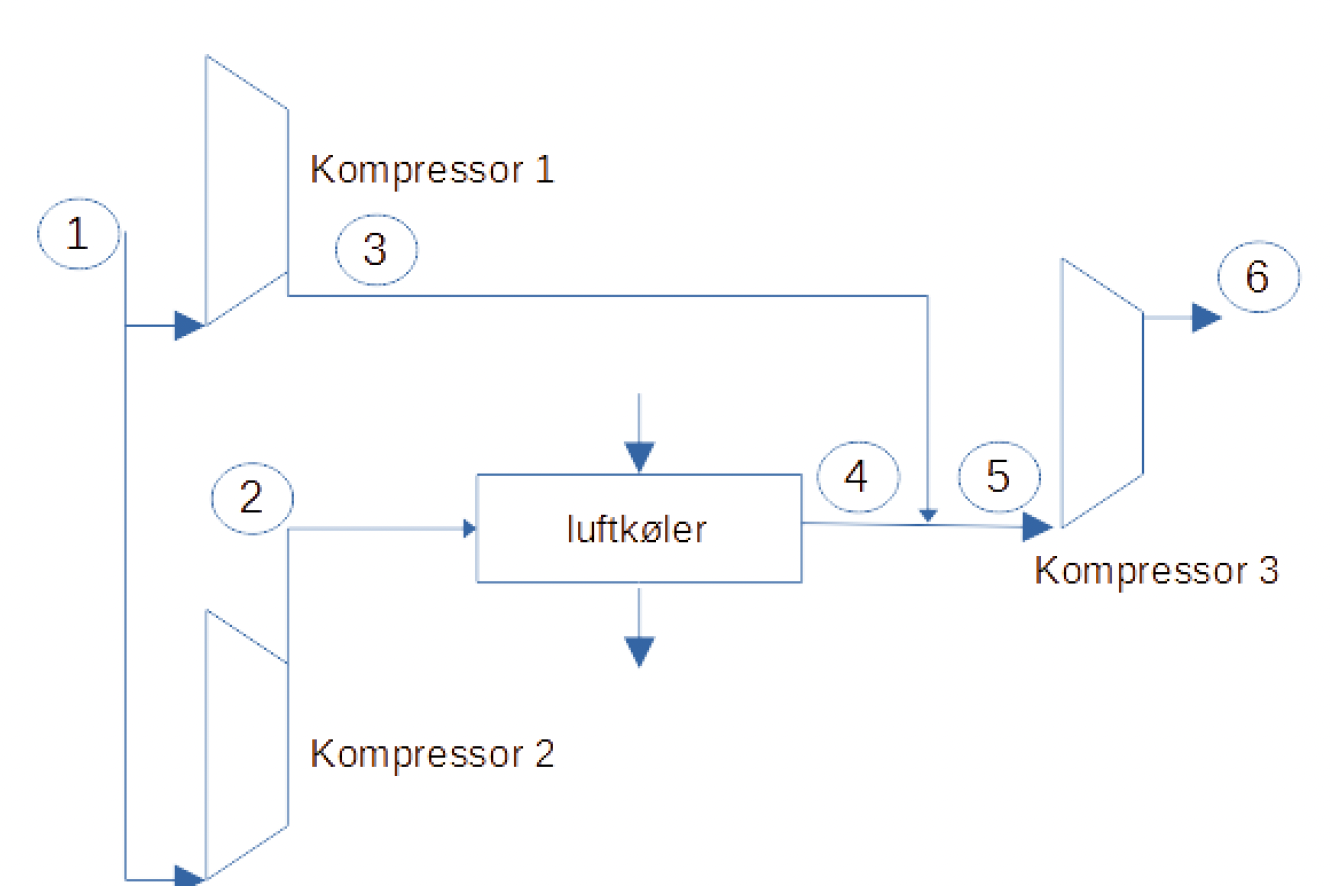
\includegraphics[width=0.5\linewidth]{./figures/e1.png}
  \caption{}
  \label{fig:e1}
\end{figure}

\opgave{1.} Forklar hvilke termodynamiske principper du lægger til grund for at regne på hvert komponent.
\bigbreak
For hele systemet bruges bl.a. kontinuitetsligningen, altså at masseflowet er konstant igennem ethvert komponent idet det antages at der ikke er nogen lægaker. Derudover benyttes også at energi er bevaret hvorved en energibalance kan opstilles på samme måde som med massen. Derudover antages at der ikke sker tryktab, varmeoverførsel m.v. igennem rørene mellem komponenterne.

Dermed kan der for hvert komponent benyttes energibalancen:
\[ 
\dot{W} + \dot{Q} = \dot{m}(h_{\mathrm{out}} - h_{\mathrm{in}}) + \Delta E_{\mathrm{kin}} + \Delta E_{\mathrm{pot}}
.\]
Hvori $\Delta E_{\mathrm{kin}}$ og $\Delta E_{\mathrm{pot}}$ udgår idet disse antages at være negligerbare. Kompressoren antages adiabatisk hvorfor det ovenstående for denne reduceres til:
\[ 
\dot{W} = \dot{m} (h_{\mathrm{out}} - h_{\mathrm{in}})
\]
og luftkøleren antages ikke at udføre et arbejde hvorfor ligningen for luftkøleren reduceres til:
\[ 
\dot{Q} = \dot{m} \left( h_{\mathrm{out}} - h_{\mathrm{in}} \right)
.\]


\opgave{2.} Forklar metode for hvordan du kan opstille en model af hele systemet.
\bigbreak
Samme punkter benyttes i EES som er angivet på tegningen. Temperatur og tryk er allerede kendt for tilstand 1, hvorfor de resterende parametre kan findes vha. stofdatakald i EES. 

Massestrømmen igennem punkt 2 og 3 er desuden begge kendte, hvorfor massestrømmen i starten også kan findes som summen af disse.

Metoden er da egentligt blot at benytte isentrop-sammenhængene såsom:
\[ 
  T[2] = T[1] \left( \frac{P[2]}{P[1]} \right)^{\frac{\kappa - 1}{\kappa}}
.\]
Hvor $\kappa = \num{1,4}$ er isentropeksponenten for luft.

\opgave{3.} Lav rimelige antagelser for de detaljer der mangler
\bigbreak
Det antages at kompressor 1 og 2 har samme trykforhold og derfor at $P[2] = P[3]$. Derudover antages at der med omgivelsestemperaturen menes $T[1]$. Ellers er koden egentligt blot stofdatakald og føromtalte isentrop-sammenhæng samt føromtalte energibalance.

\opgave{4.} Opstil en EES-model for systemet med idealiserede komponenter.
\bigbreak
Med afsæt i ovenstående antagelser og metode er følgende EES-kode blevet konstrueret:
\begin{verbatim}
  m_dot[1] = m_dot[2] + m_dot[3]
  m_dot[2] = 2
  m_dot[3] = 3
  m_dot[4] = m_dot[2]
  m_dot[5] = m_dot[1]
  m_dot[6] = m_dot[1]

   
  T[1] = 293
  P[1] = 101
  s[1] = entropy(Air_ha; T=T[1]; P=P[1])
  h[1] = enthalpy(Air_ha; T=T[1]; P=P[1])
   
  k = 1,4
   
  P[3] = 500
  T[3] = T[1] * (P[3]/P[1])^((k-1)/k)
  s[3] = entropy(Air_ha; T=T[3]; P=P[3])
  h[3] = enthalpy(Air_ha; T=T[3]; P=P[3])
   
  W_1 = m_dot[3] * (h[3] - h[1])
   
  P[2] = P[3]
  T[2] = T[1] * (P[2]/P[1])^((k-1)/k)
  s[2] = entropy(Air_ha; T=T[2]; P=P[2])
  h[2] = enthalpy(Air_ha; T=T[2]; P=P[2])
   
  W_2 = m_dot[2] * (h[2] - h[1])
   
   
  T[4] = T[1] + 5
  P[4] = P[2]
  s[4] = entropy(Air_ha; T=T[4]; P=P[4])
  h[4] = enthalpy(Air_ha; T=T[4]; P=P[4])
   
  Q_cool = m_dot[2] * (h[2] - h[4])
   
   
  h[5] = (m_dot[2] * h[2] + m_dot[3] * h[3])/m_dot[1]
  P[5] = P[4]
  T[5] = temperature(Air_ha; h=h[5]; P=P[5])
  s[5] = entropy(Air_ha; T=T[5]; P=P[5])
   
  P[6] = 1000
  T[6] = T[5] * (P[6]/P[5])^((k-1)/k)
  s[6] = entropy(Air_ha; T=T[6]; P=P[6])
  h[6] = enthalpy(Air_ha; T=T[6]; P=P[6])
\end{verbatim}


\opgave{5.} Beregn den tilførte effekt for kompressor 2.
\bigbreak
Med afsæt i EES koden ovenfor er den tilførte effekt for kompressor 2 regnet til $W_2 = \qty{343,2}{kW}$. 

\opgave{6.} Beregn den afgivne effekt i luftkøleren.
\bigbreak
Med afsæt i EES koden ovenfor er den afgivne effekt i luftkøleren regnet til $Q_{\mathrm{cool}} = \qty{331,3}{kW}$

\opgave{7.} Opstil et skema med relevante tilstandsstørrelser.
\bigbreak
EES har på baggrund af koden fra opgave 4 produceret tabellen på \textbf{\autoref{fig:e2}}.
\begin{figure} [ht]
  \centering
  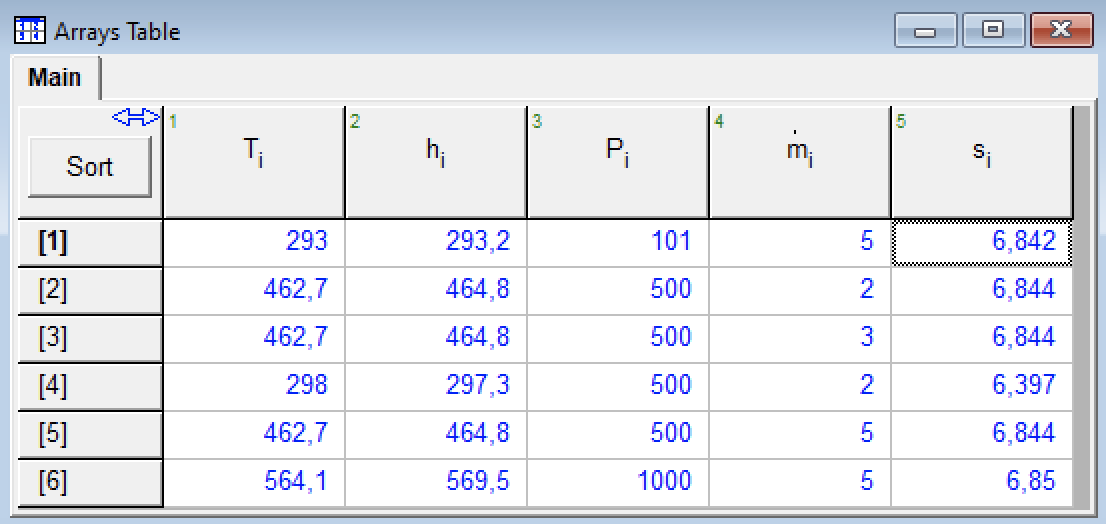
\includegraphics[width=0.5\linewidth]{./figures/e2.png}
  \caption{}
  \label{fig:e2}
\end{figure}


\section{Opvarmning af luft}
\opgave{1.} Tegn en systemskitse.
\bigbreak
\begin{figure}[ht]
  \centering
  \incfig[0.8]{e3}
  \caption{}
  \label{fig:e3}
\end{figure}

\opgave{2.} Hvilke relevante antagelser kan de gøre?
\bigbreak
Det antages først og fremmest at der intet tryktab er over varmeveksleren. Derudover antages som sædvanligt at der ikke er varmetab eller massetab til omgivelserne. 

\opgave{3.} Opstil en beregningsmodel.
\bigbreak
Følgende beregnignsmodel er opstillet i EES:
\begin{verbatim}
  T[1] = 20
  rh[1] = 0,9
  V_dot = 300
  P = 101
   
  X[1]=humrat(AirH2O;T=T[1];R=rh[1];P=P)
   
  h[1]=enthalpy(AirH2O;T=T[1];w=X[1];P=P)
   
  rho[1]=density(AirH2O;T=T[1];w=X[1];P=P)
   
  T[2] = 40
   
  X[2] = X[1]
  h[2]=enthalpy(AirH2O;T=T[2];w=X[2];P=P)
   
   
  Vdot_s = V_dot / 3600,0
   
  m_dot_ha = rho[1] * Vdot_s          //massestrøm fugtig luft
  m_dot_da = m_dot_ha / (1 + X[1])    //massestrøm tør luft
   
  Q_dot = m_dot_da * (h[2] - h[1])
\end{verbatim}

\opgave{4.} Hvad er effektbehovet?
\bigbreak
Af EES-koden ovenfor kan regnes at det kræver $\dot{Q} = \qty{2}{kW}$ kontinuert tilført varmeeffekt at opvarme luften. Her er formlen for varmetilførslen i en varmeveksler brugt som i sidste opgave:
\[ 
  \dot{Q} = \dot{m} \cdot \left( h[2] - h[1] \right)
.\]


\opgave{5.} Hvilken type varmeveksler vil du vælge?
\bigbreak
Jeg ville nok vælge at benytte en modstrøms pladevarmeveksler. Korrosionskravene virker ikke til at være enormt høje såfremt det blot er rent vand og luft der kommer forbi varmeveksleren, specielt idet temperaturen ikke er højere. Varmeveksleren anbefales at sættes i modstrøm for at maksimere den effektive temperaturforskel mellem fjernvarmevandet og luften. Varmeveksleren skal i øvrigt være dimensioneret til at kunne yde mindst de påkrævede $\dot{Q} = \qty{2}{kW}$. 


\section{Afkøling af luft}

\opgave{1.} Tegn en systemskitse
\begin{figure}[ht]
  \centering
  \incfig[1]{e31}
  \caption{}
  \label{fig:e31}
\end{figure}

\opgave{2.} Indtegn luftens afkølingsprocess i et $hx$-diagram.
\bigbreak
Her er genbrugt store dele af EES-koden fra sidste hovedopgave
\begin{verbatim}
  T[1] = 40
  rh[1] = 0,9
  V_dot = 300
  P = 101
   
  X[1]=humrat(AirH2O;T=T[1];R=rh[1];P=P)
   
  h[1]=enthalpy(AirH2O;T=T[1];w=X[1];P=P)
   
  rho[1]=density(AirH2O;T=T[1];w=X[1];P=P)
   
  T[2] = 20
   
  X[2]=humrat(AirH2O;T=T[2];R=1;P=P)       //Mætningsfugt R=1
  h[2]=enthalpy(AirH2O;T=T[2];w=X[2];P=P)
   
   
  Vdot_s = V_dot / 3600,0
   
  m_dot_ha = rho[1] * Vdot_s          //massestrøm fugtig luft
  m_dot_da = m_dot_ha / (1 + X[1]) //massestrøm tør luft
   
  Q_dot = m_dot_da * (h[2] - h[1])
\end{verbatim}
Bemærk dog at $X[2]\neq X[1]$ i dette tilfælde da nedkølingen vil resultere i at vand udfældes, dermed er fugtforholdet i sluttilstanden blot tilsvarende mætning. 

Med afsæt i denne EES-kode er dette diagram produceret:
\begin{figure} [ht]
  \centering
  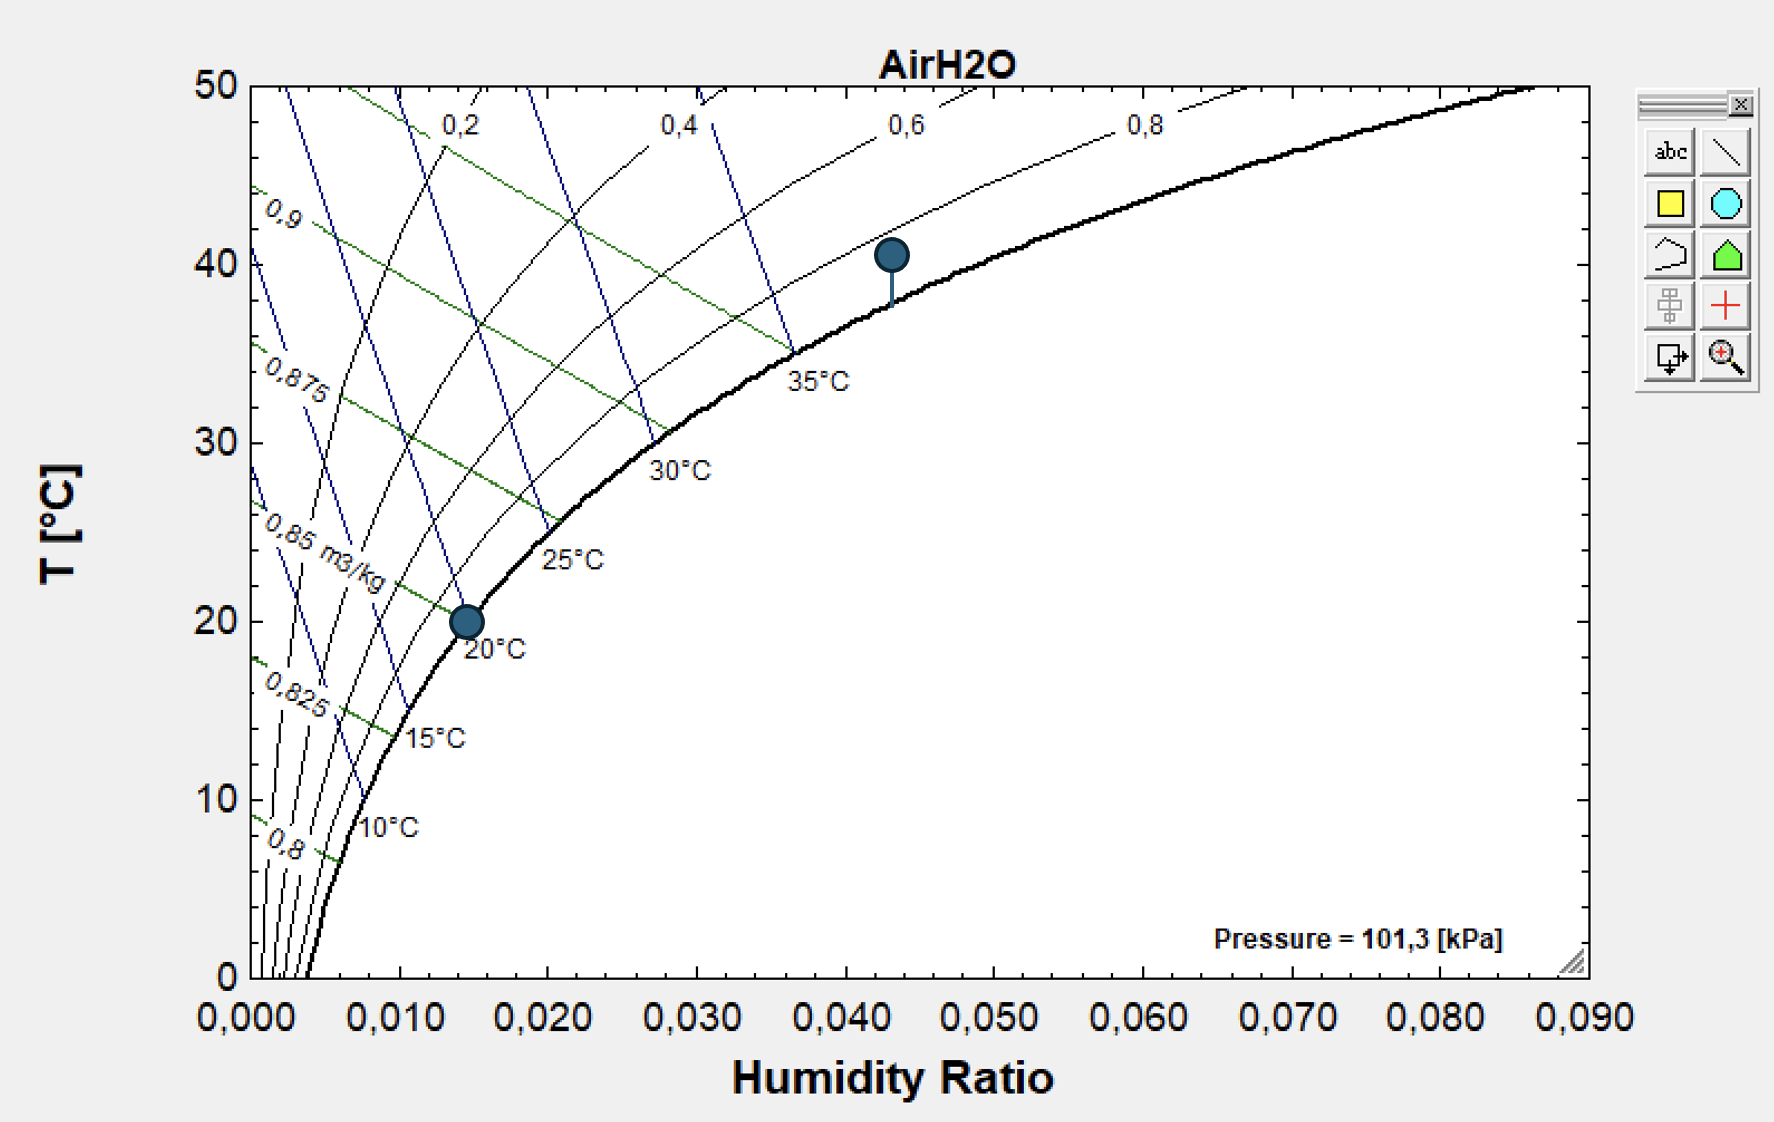
\includegraphics[width=0.5\linewidth]{./figures/e6.png}
  \caption{}
  \label{fig:e6}
\end{figure}

Bemærk her at vandets processvej er lodret ned indtil mætningskurven rammes, hvorefter vandet følger denne.

\opgave{3.} Hvad er effektbehovet?
\bigbreak
Med afsæt i ovenstående EES-kode er effektbehovet regnet til $\dot{Q} = \qty{8,356}{kW}$.


\section{Tryk i en vandflaske der fryses}

\opgave{1.} Hvad bliver trykket i flaske 1?
\bigbreak
Vi antager at den givne volumen af vand er fyldt i flasken ved stuetemperatur ($T[1] = \qty{20}{\celsius}$) og at vi måler trykket netop idet det sidste vand fryser ved $T[2] = \qty{0}{\celsius}$. Først findes densiteten af vandet og luften i starttilstanden for at finde deres respektive masser. Massen ændres nemlig ikke af en frysning hvorfor denne er konstant. Efter massen er fundet kan det resulterende tryk i sluttilstanden findes idet der her blot kan regnes den anden vej tilbage til et tryk.

På baggrund heraf er følgende EES-kode konstrueret:
\begin{verbatim}
  V_flaske_L = 0,32
  V_flaske_m3 = V_flaske_L/1000
   
  P[1] = 101
  T[1] = 20 //starttemperatur
  T[2] = 0 // frysetemperatur
   
  V_vand_L = 0,25
  V_vand_m3 = V_vand_L/1000
   
  V_luft[1] = V_flaske_m3 - V_vand_m3
   
  rho_air[1] = density(Air_ha; T=T[1]; P=P[1]) // luftens densitet ved starten
   
  m_air = rho_air[1] * V_luft[1] //luftens masse i starten
   
  rho_vand[1] = density(Water; T=T[1]; P=P[1]) // vandets densitet i starten
  m_water = rho_vand[1] * V_vand_m3              // massen af vandet
   
  P[2] * V_air[2] = m_air * 0,287 * T[2]      // Idealgasligningen
   
  V_air[2] = V_flaske_m3 - m_water / density(Ice; T = T[2]; P = P[2])  // volumen tilbage til luft efter frysning
\end{verbatim}
Dermed fås at trykket i flasken efter frysningen er \qty{138}{kPa}. 

\opgave{2.} Hvad bliver trykket i flaske 2?
\bigbreak
Her kan samme EES-kode langt hen ad vejen benyttes dog skal linje 8 ændres fra:
\begin{verbatim}
  V_vand_L = 0,25
\end{verbatim}
til
\begin{verbatim}
  V_vand_L = 0,2
\end{verbatim}
Dermed fås trykket efter frysningen til $\qty{111}{kPa}$.

\opgave{3.} Forklar forskellen.
\bigbreak
Forskellen mellem de to trykmålinger opstår idet der er forskellige mængder vand i flaskerne fra starten af. Vand ændrer (som de fleste andre stoffer) densitet idet det gennemgår en fasetransition. Idet vandets densitet ændres mens dets masse fastholdes må dets volumen ligeledes ændres.

Når vandets volumen ændres ændres også volumenet som luften har mulighed for at udfylde. Denne ændring af luftens tilgængelige volumen er årsag til trykændringen. Idet der er mere vand i flasken i det første tilfælde vil det også udvide sig tilsvarende mere som resultat af frysningen.

For vand gælder i øvrigt at det er et af de få stoffer der udvider sig idet det fryser, hvorfor trykket i flasken stiger under frysningen. Dette er årsagen til at dåser sprænger i luften, hvis man glemmer dem i en fryser. 

\section{Sammenligne tørretumblere}

\opgave{1.} Hvilken model bruger mest strøm?
\bigbreak
\textit{Whirlpool}-modellen har energimærke A++ medens \textit{Logik}-modellen kun har energimærke B. Whirlpool-modellen bruger kun omtrent halvt så meget strøm som Logik-modellen både målt på årsbasis og på en enkelt vask. Dette er en ret betydelig forskel.

\opgave{2.} Forklar opbygningen af de to modeller og forskellene -- tegn systemdiagram.
\bigbreak
Nedenfor ses de to systemdiagrammer.
\begin{figure}[ht]
  \centering
  \incfig[0.75]{e4}
  \caption{Logik-modellen}
  \label{fig:e4}
\end{figure}
\begin{figure}[ht]
  \centering
  \incfig[0.75]{e5}
  \caption{Whirlpool-modellen}
  \label{fig:e5}
\end{figure}

\opgave{3.} Forklar hvorfor den ene bruger mindre energi end den anden.
\bigbreak
Logik-modellen varmer op udelukkende ved brug af resistiv opvarmning. Meget af denne varme går tabt til omgivelserne og der gøres ingen forsøg på at genindvinde varmen efter brug. Whirlpool-modellen derimod benytter en varmepumpe til at genindvinde varmen, hvorfor en stor del af varmeregningen kan spares.

Desuden er tørretiden næsten 7 gange så lang for Logik-modellen som for whirlpool. Dette kan skyldes at logik muligvis tørrer tøjet mere end whirlpool-modellen, men det kan også skyldes mere effektiv styring af tørringsprocessen i den mere moderne maskine. 

\opgave{4.} Er der potentiale for yderligere forbedringer og i givet fald hvordan?
\bigbreak
Specielt for Logik-modellen er det nemt at hæve effektiviteten -- her kunne man med fordel lade sig inspirere af Whirlpool-modellens varmepumpe. 

Derudover kan man altid optimere på udformningen af eksempelvis tromlen for at sikre bedre luftgennemstrømning samt øget isolering.

\end{document}
